% !TEX root =  paper.tex
\section{DigiTaps Game}
\label{sec:digitaps}

Since the preliminary evaluation of the DigiTaps code shows promising results, a more rigorous study is needed to evaluate the Espresso and the Cappuccino methods. The Espresso and the Cappuccino methods have been evaluated in a lab study as presented in \cite{Azenkot:2013}. The study compared the performance of the Espresso method to the performance of the Cappuccino method when using the methods with different kinds of feedback, only haptic feedback and both haptic and audio feedback. With both the audio and haptic feedback on, the participants entered the numbers at a rate of 0.82 digits per second and 0.78 digits per second using the Cappuccino method and the Espresso method, respectively. The participants achieved a low mean uncorrected error rate of 2.17\% and 2.22\% using the Cappuccino method and the Espresso method, respectively. The longitudial lab study's results agreed with the preliminary evaluation that the Espresso method is fast and accurate.
\par
Even though the lab study and the preliminary evaluation showed that the participants entered numbers with a fast speed and accurately using the DigiTaps codes, it does not reflect the real use of the gestures in a real-world setting. We want to design a user study that simulate real world use of the gestures. Hence, we adopted the user study model presented in \cite{Henze:2011} to conduct our user study in the wild. We developed DigiTaps Game for conducting number entry method user studies in the wild. The game is designed to emphasize the number entry speed and the accuracy of inputting numbers, which we considered as the prominent performance factors in real world use of the gestures.
\par
The DigiTaps game collects touch events that the player performs while they are playing the game. We collect the touch events for evaluating the Espresso and the Cappuccino methods. We expose the DigiTaps game to a large number of players by distributing the game via the Apple App Store.

\subsection{Flow of DigiTaps}
% describes the game states
The first screen shown to the player after launching DigiTaps is the main menu of the game as (see Figure \ref{startscreen}). This screen consists of three choices for the player to choose
  \begin{enumerate*}[(1) ]
    \item Tutorial, 
    \item Start Game, 
    \item Leaderboard.
  \end{enumerate*}
  Selecting different button leads to different modes of the DigiTaps game and leads to different screens that the player visits.
  
\begin{figure}[ht!]
  \centering
  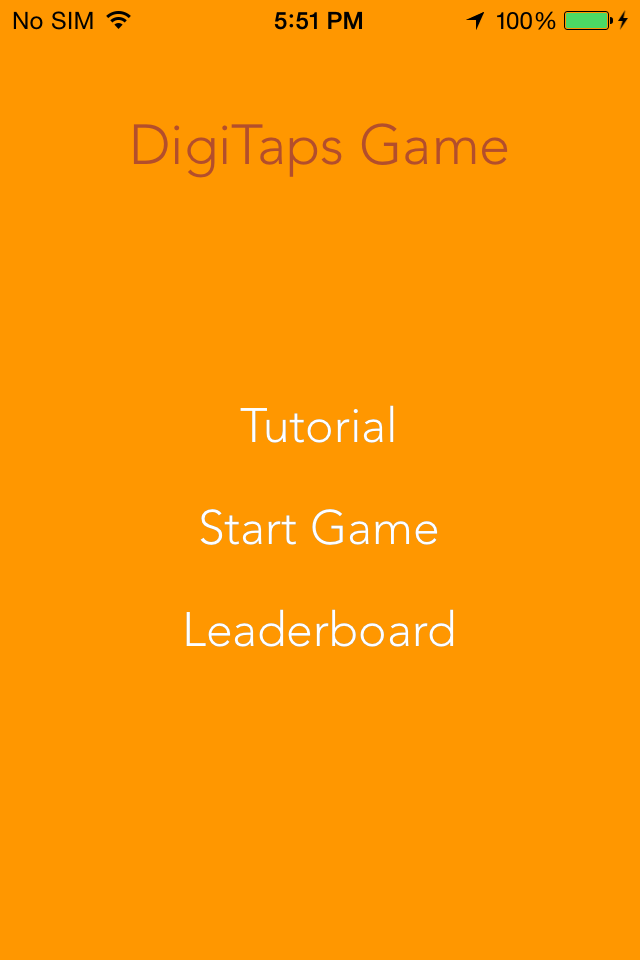
\includegraphics[width=0.5\textwidth]{figures/start.png}
  \caption{Main menu and the first screen of DigiTaps}
  \label{startscreen}
\end{figure}

\subsubsection{Tutorial}
    We provide tutorials for the players to get started with the DigiTaps codes. Each tutorial consists of the description of the code and the practice mode for the code. There are three tutorials total. The first tutorial is the overall description of the game. It describes the main gestures of the game such as long-press to submit the number. The two other tutorials describe the DigiTaps codes. In each DigiTaps code description screen, a table describing how the gestures map to the DigiTaps codes is provided. The practice screen allows the player to try out the gestures they learned in the description screen. The practice screen gives the user feedback on the action the player just perform. For example, if the player tap the screen with three fingers, the screen shows that it is a three-finger tap (see the rightmost state in figure \ref{tutorial}).

\begin{figure}[ht!]
  \centering
  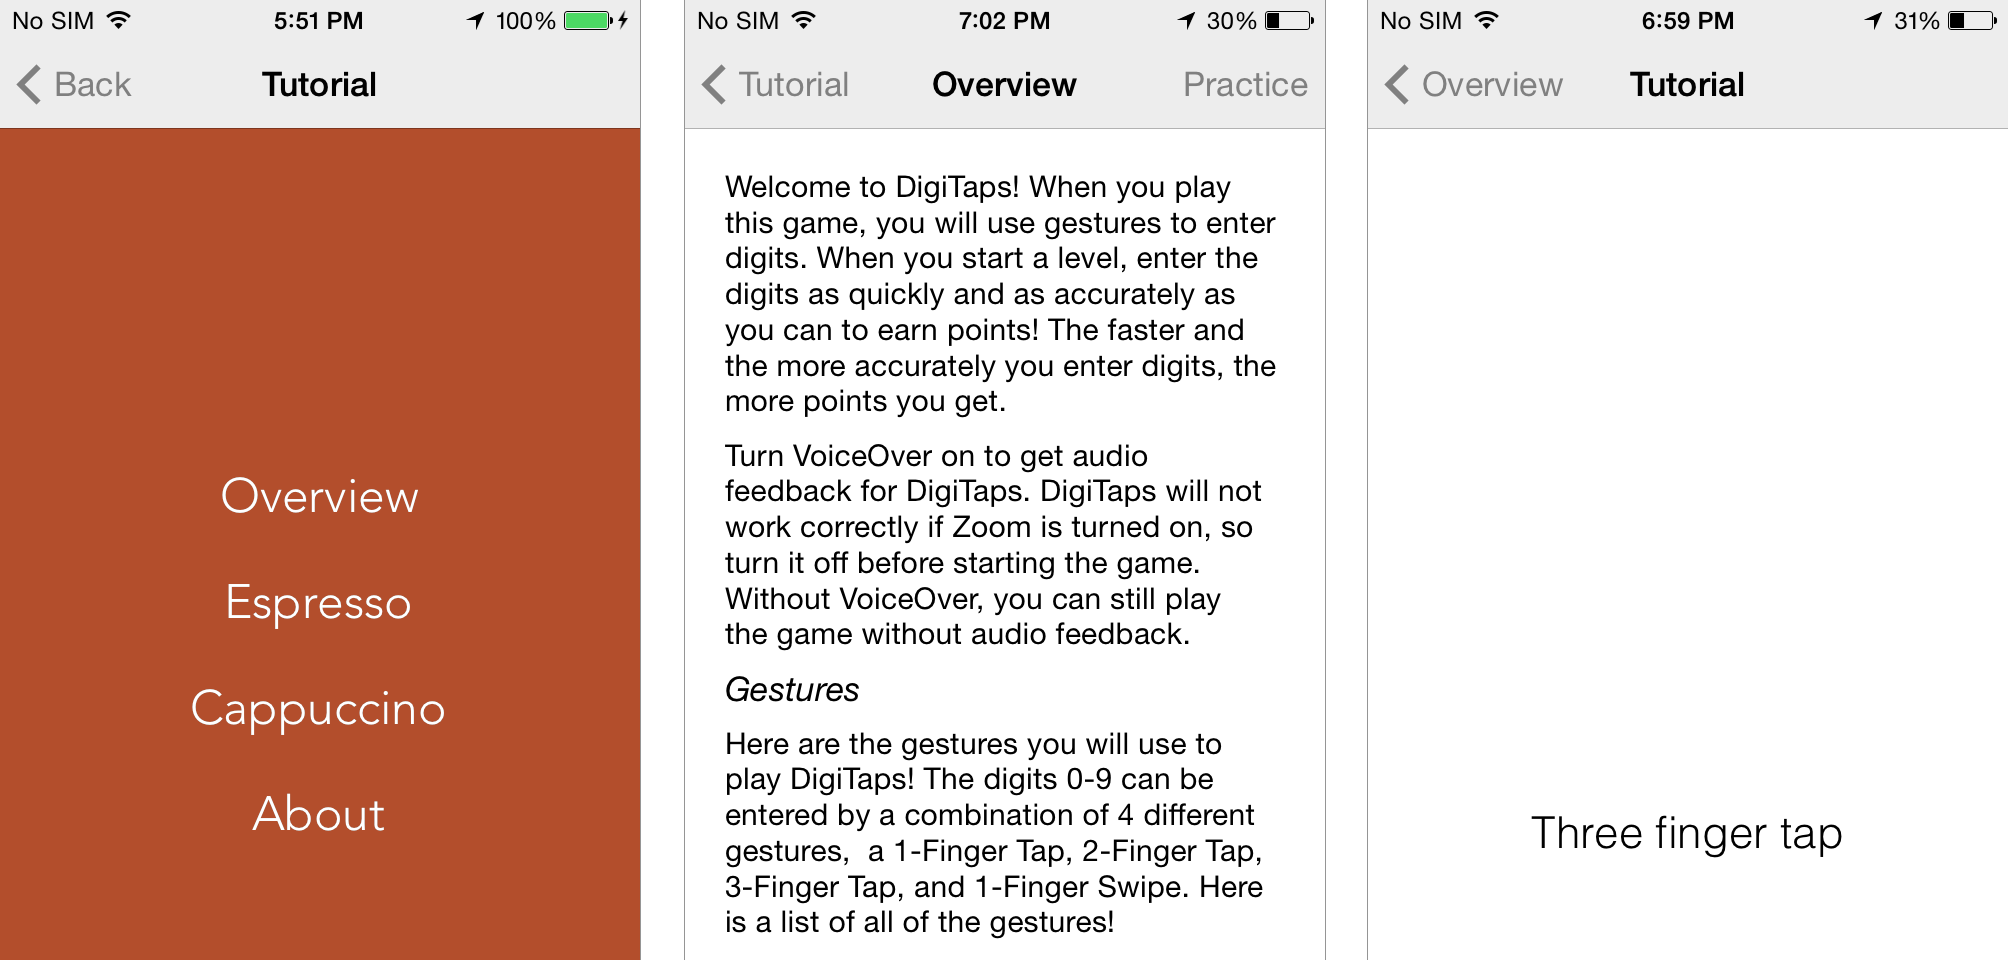
\includegraphics[width=1.0\textwidth]{figures/tutorial.png}
  \caption{The state on the left shows the options the player can choose to learn about. The state in the middle is an example of a tutorial page where descriptions are provided. The state on the right is an example of a practice screen.}
  \label{tutorial}
\end{figure}

\subsubsection{Game Play}
There are 4 main screens
    \begin{enumerate*}[(1) ]
      \item a DigiTaps method selection screen, 
      \item a level selection screen, 
      \item a game play screen, and
      \item a summary screen.
    \end{enumerate*}
    At the method selection screen, the DigiTaps game lets the player chooses either the Espresso method or the Cappuccino method. The player will use the method chosen to enter numbers through out the game. After the method has been chosen, the player has to choose a level to start playing the game, indicated by the red arrow in figure \ref{gameplay} from the top row to the leftmost state on the second row.
\par    
At this point, the game play screen slides in and show the first number to the player (see the leftmost state of the second row in figure \ref{gameplay}). The player performs the gestures to enter the number shown on the screen. To submit the number, the player has to tap and hold that finger on screen with one finger until a ringing or a buzz sound occurs. The sound means that the number has been submitted. A ringing sound indicates that the number input was correct, and the buzz sound indicates an incorrect attempt. The player, then, advances to the next number. The player has to enter 10 numbers per level and the number of digits per number varies based on the level. The numbers starts with 3 digits per number at level 1 and the number of digits increases by one digit as the player progresses through the levels. At the last level, level 5, each number is 7 digits long.
\par
After entering all the numbers required, the summary screen appears. The summary screens provides the player's performance on that level. The information includes the points earned, the accuracy and the average time per digit. On this screen, the player has the option to advance to the next level, replay the same level or quit to the start menu as (see the last state of figure \ref{gameplay}).

\begin{figure}[ht!]
  \centering
  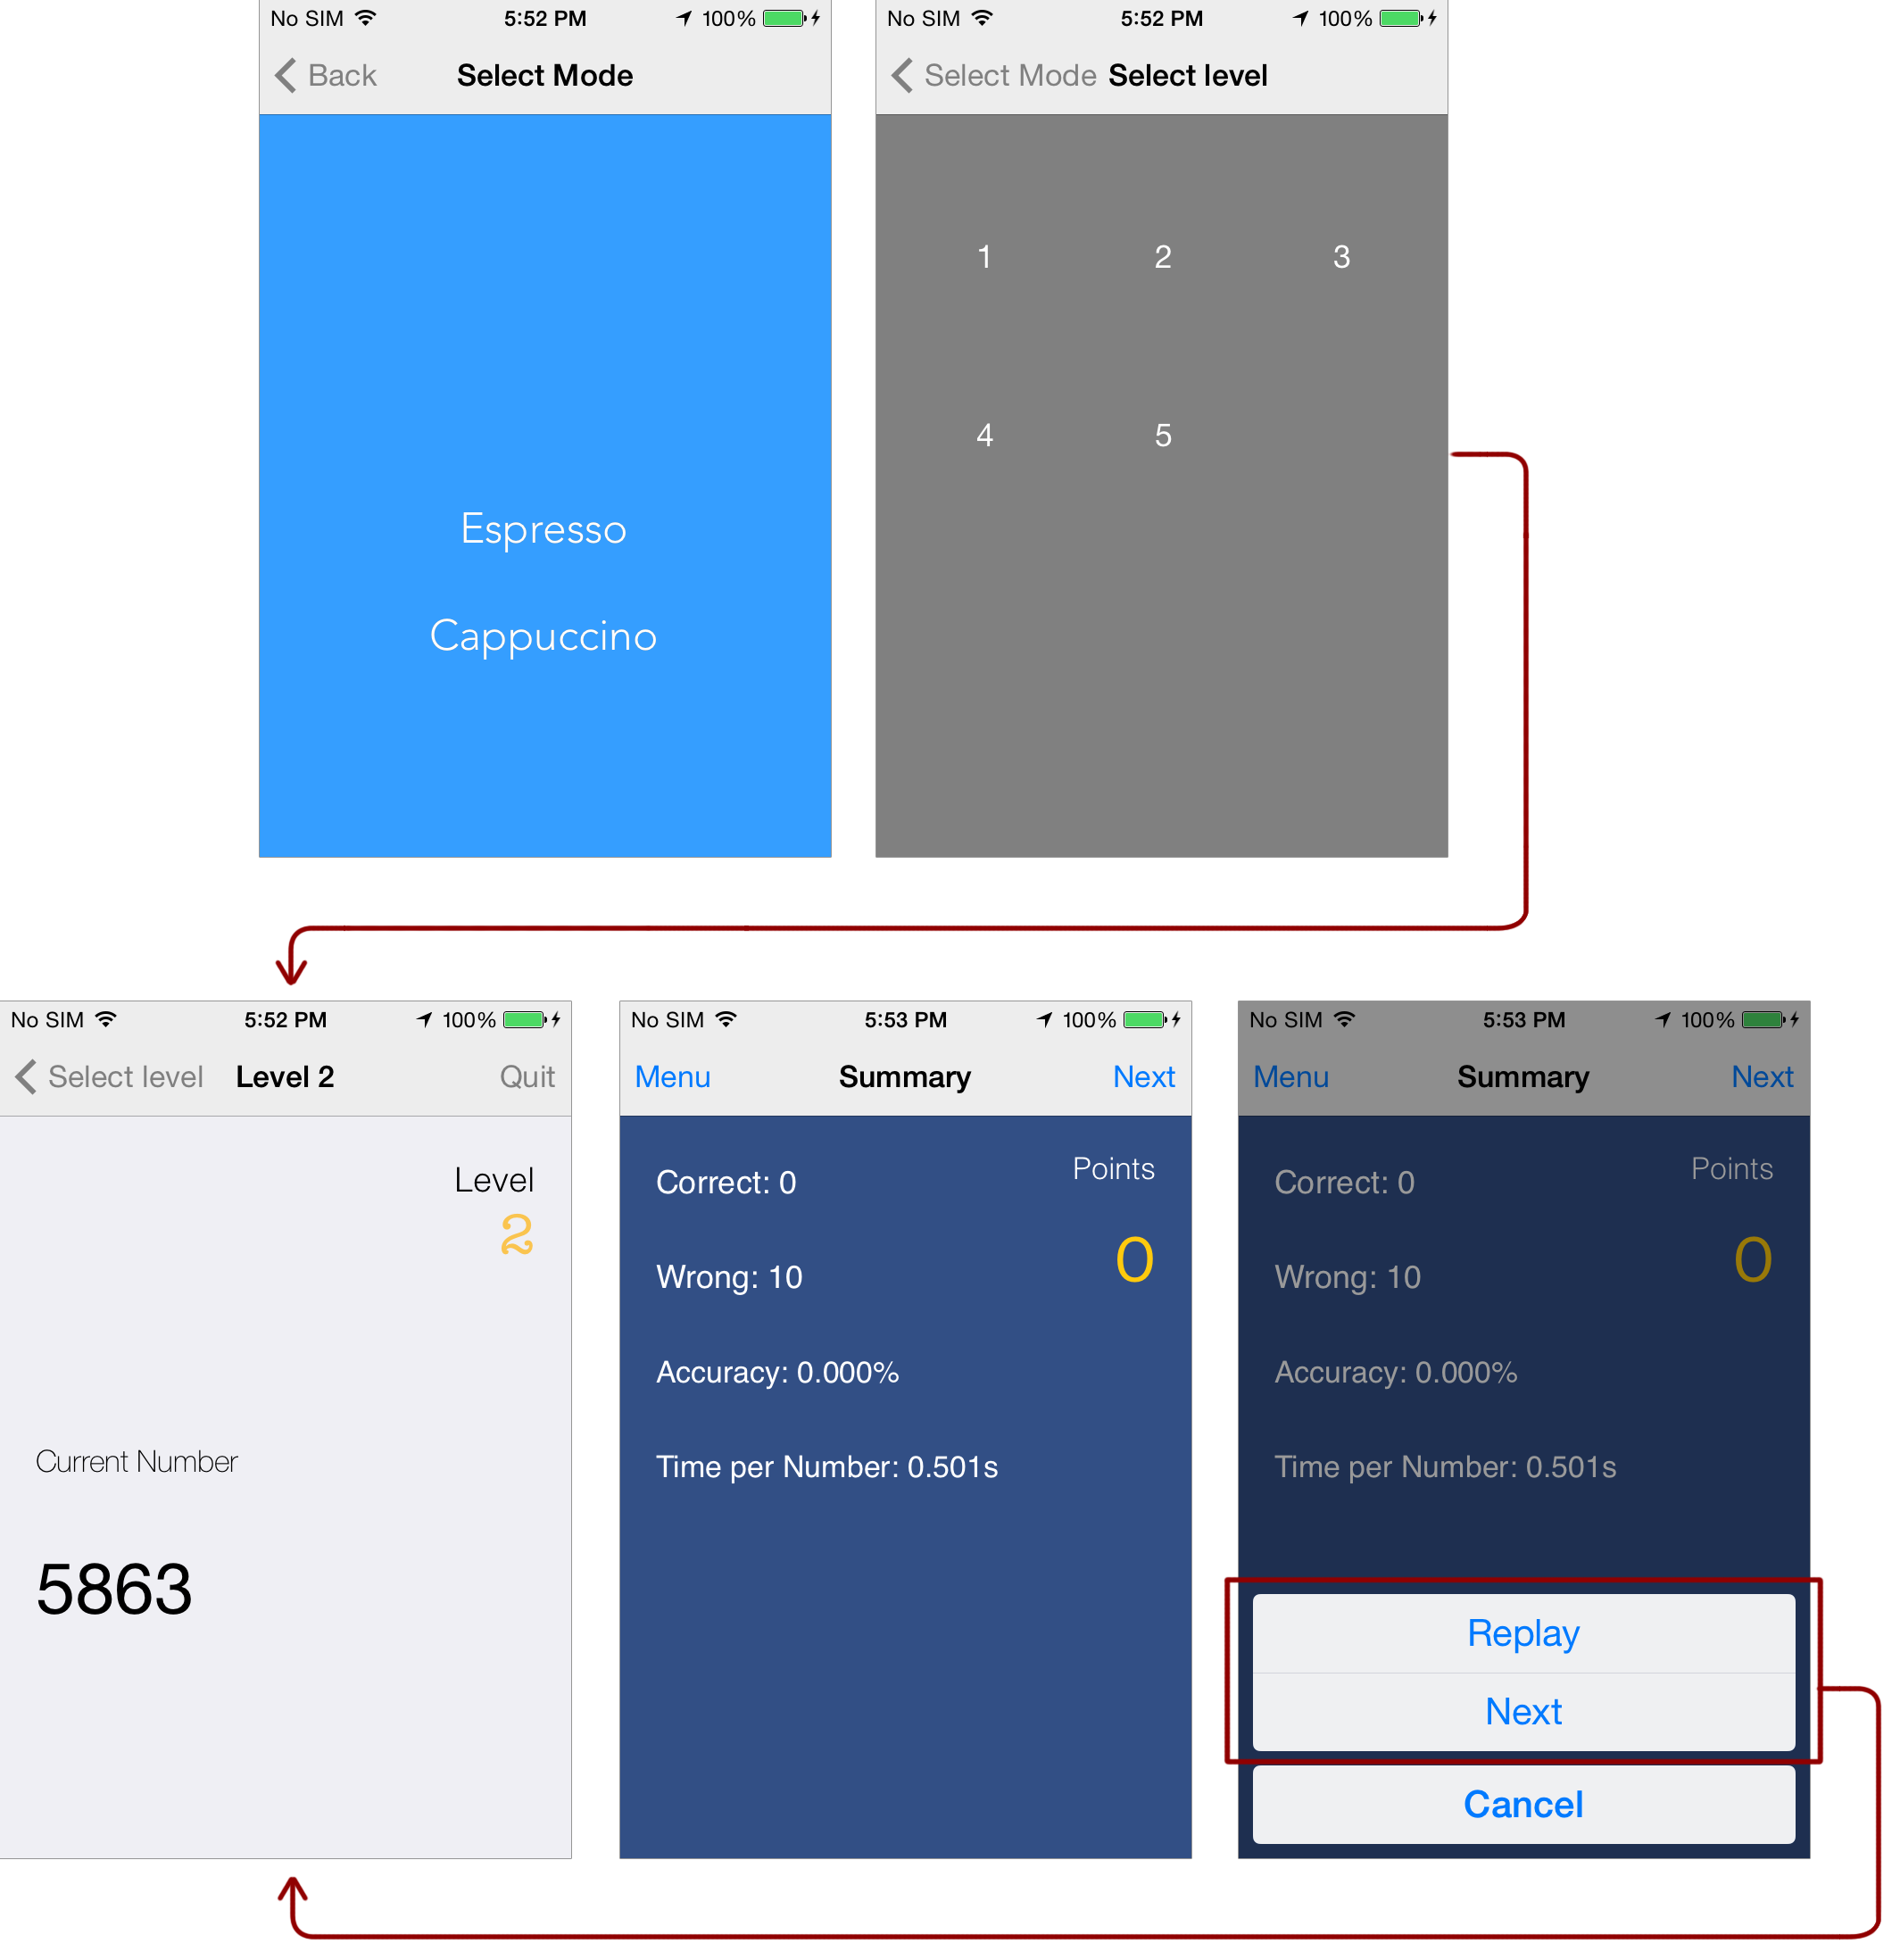
\includegraphics[width=1.0\textwidth]{figures/gameplay.png}
  \caption{Shows the state diagram of DigiTaps gameplay mode.}
  \label{gameplay}
\end{figure}
    
\subsubsection{Leaderboard and Scoring}
    To provide the players with competition, we include Apple's Leaderboard into DigiTaps. The Leaderboard ranks the player's score with other players around the world who plays the DigiTaps game and uses Apple's Game Center. Players are being ranked by the scores they achieved in the game (see figure \ref{leaderboard}). Players can compare their scores with other players' scores and see how well they are doing.
    \par
    We compute the points based on the player's speed and accuracy. Each number in a level contributes to the overall points in a level. If the player incorrectly enters a number, the player will get zero points for that number. If the player enters the number correctly, the score for that number will be computed. The score is computed using the following formula.
    \begin{align*}
      score &= \frac{\mbox{expected time used}}{\mbox{actual time used}} \times \mbox{baseline}
    \end{align*}
    In other words, if the player enters the number faster than what the game has expected, the game will reward the player with a higher score than the baseline. In contrary, if the player enters the number slower than what the game has expected, the game will penalize the player with a lower score. The baseline is an arbitrary number.
    
\begin{figure}[h!]
  \centering
  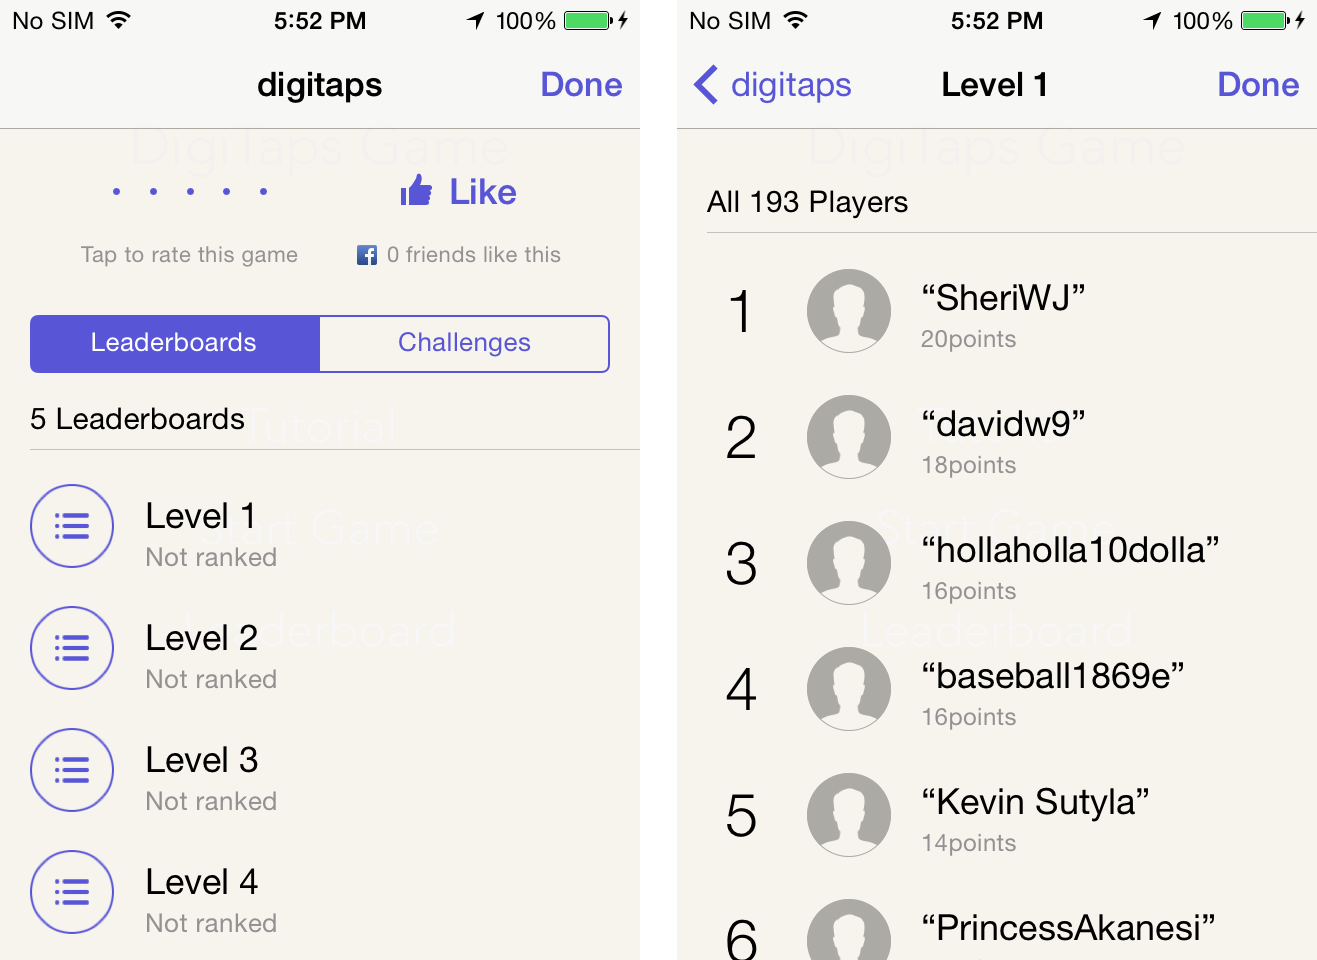
\includegraphics[width=1.0\textwidth]{figures/leaderboard.png}
  \caption{The state on the left shows the leaderboard of each level. The state on the right shows the rankings of the first six places for level 1 with their respective points.}
  \label{leaderboard}
\end{figure}

\subsection{Interaction Gestures}
In addition to the DigiTaps gestures described in the DigiTaps code section, the DigiTaps game uses two other gestures for players to interact with the game. The first gesture is two-finger swipe in any direction. This gesture does two actions in the game. If the player already input numbers into the game, two-finger swipe in any direction activates the backspace action. Since the number initially shown on the screen disappears when the player starts entering the numbers, we use two-finger swipe in any direction to repeat the number. DigiTaps game repeats the number by reading the number to the player again and shows the numbers on the screen again.
\par
The second special gesture is the long-press gesture. This gesture is used for advancing to the next number in the level or if there is no more number on that level, this gesture takes the player to the summary screen. When the player finishes inputting the given number, the player holds one-finger down on the screen until there is a bell ring or a buzz sound from DigiTaps. The sound indicates that the game has advanced to either the next number or the summary screen. The bell sound indicates a correct attempt and the buzz sound indicates a failed attempt.

\subsection{Data Collection}
In order to conduct the user study, we collect two different kinds of information from the players, the players' demographics and the touch events that the players performed. The demographics information includes the player's age, gender, experience with accessibility in iOS. Each player is uniquely identify with an identification number. However, we cannot trace back to who the actual player was. This identifier is used to match the player to the other information of this player that collected.
\par
The touch events that the players performed in the game is also recorded. In each of these touch events, we record the number entered and the timestamp when the event occurred. Furthermore, we recorded the state of the game such as when the game starts, the level finishes, and the number is inputted. We recorded the numbers presented to the players and the numbers that the players entered. We used this information to measure the accuracy of the players.
\par
Using the information collected, we can gain some insight on how the players behave in the game. More importantly, we can evaluate the speed and the accuracy of the players performing the gestures by analyzing the players' data.